\documentclass[11pt,letterpaper,final] {article}

%%%%%%%%%%%%%%%%%%%%%%%%%%%%%%
% Packages
%%%%%%%%%%%%%%%%%%%%%%%%%%%%%%

	\usepackage[margin=1in]{geometry}
	\usepackage{amsmath}
	\usepackage{amsfonts}
	\usepackage{fancyhdr}
	\usepackage{graphicx}
	\usepackage{scrextend}
	\usepackage{apacite}
	% \usepackage{tikz}
	% \usepackage{setspace}
	% \usepackage{multicol}

%%%%%%%%%%%%%%%%%%%%%%%%%%%%%%
% Page styling
%%%%%%%%%%%%%%%%%%%%%%%%%%%%%%
	
	%%%%%%%%%%%%%%%%%%%%
	% Headers and footers
	%%%%%%%%%%%%%%%%%%%%
	
	\pagestyle{fancy}
	\renewcommand{\headrulewidth}{0pt}
	\fancyhead{}
	\fancyfoot{}
	\lhead{Wetherill}
	\rhead{\thepage}
	
	%%%%%%%%%%%%%%%%%%%%
	% Graphics path
	%%%%%%%%%%%%%%%%%%%%
	
	\graphicspath{{./assets/}}
	
	%%%%%%%%%%%%%%%%%%%%
	% Frontmatter
	%%%%%%%%%%%%%%%%%%%%
	
	% \title{The Title}
	% \author{The Author}
	% \date{\today}
	
	

%%%%%%%%%%%%%%%%%%%%%%%%%%%%%%
% Custom definitions
%%%%%%%%%%%%%%%%%%%%%%%%%%%%%%
	% Easy scientific notation
	\newcommand{\e}[1]{\ensuremath{\times 10^{#1}}}
	
	% Textual subscripts
	\newcommand{\sub}[1]{\ensuremath{_{\text{#1}}}}
	
	% Textual superscripts
	\newcommand{\super}[1]{\ensuremath{^{\text{#1}}}}
	
	\newenvironment{exercise}[2][Exercise]{\begin{trivlist}
	\item[\hskip \labelsep {\bfseries #1}\hskip \labelsep {\bfseries #2.}]}{\end{trivlist}}
	
	\newenvironment{problem}[2][Problem]{\begin{addmargin}[0.5in]{0em} \begin{trivlist}
	\item[\hskip \labelsep {\bfseries #1}\hskip \labelsep {\bfseries #2.}]}{\end{trivlist}\end{addmargin}}


\begin{document}
% \maketitle

\noindent Christopher Wetherill \\
TBMH 5054 \\
Midterm Exam \\[1cm]

\begin{exercise}[Exercise]{1} A 32-year-old woman presented a severe case of pseudomembranous colitis due to infection with antibiotic-resistant \textit{C. diff}. Exhausting other options, she underwent a fecal transplant, donated from her then-obese daughter. Although cured of her \textit{C. diff} infection, the patient subsequently gained 36 lbs. and is now classified as obese.\\

	\begin{problem}[Problem]{A} Explain the pathology of pseudomembranous colitis.
	
	Pseudomembranous colitis is an inflammation of the large intestine resulting from infection with \textit{Clostridium difficile} bacterium \cite{Moreno:2013}.\\
	
	\end{problem}
	
	\begin{problem}[Problem]{B} Explain how \textit{Clostridium difficile} can cause diarrhea.
	
	\textit{C. difficile} colonizes the large intestine of humans. From here, diarrhea is induced through the activity of toxin A (TcdA) and toxin B (TcdB). Specifically, these toxins inactivate $\rho$ GTPases through enzymatic glucosylation of a threonine residue. In turn, this induces actin depolymerization and disruption of the actin cytoskeleton, ultimately resulting in cell apoptosis. These dead epithelial cells are then sloughed off and present as watery stool or diarrhea \cite{Burke:2014}.\\
	
	\end{problem}
	
	\begin{problem}[Problem]{C} What is fecal microbiota transplant?
	
	Fecal microbiota transplantation refers to a procedure in which healthy donor feces is instilled in a patient with GI microbial dysbiosis. This procedure aims to re-establish the normal composition of a healthy gut microbiome and, by establishment of commensal microbial colonies, to restore normal healthy gut function and inhibit activity of pathogenic bacteria \cite{Vecchio:2014}.\\
	
	\end{problem}
	
	\begin{problem}[Problem]{D} Provide the rationale for selecting the donor for the fecal microbiota transplant.
	
	A healthy family member or friend is typically the preferred donor for a fecal microbiota transplant. Further, to minimize the risk of transmission of unknown pathogens, potential donors' travel history, sexual behavior, previous medical procedures and operations, and blood transfusions should be noted. It has been shown that there is a slightly higher rate of successful disease resolution following transplant from related donors (93\%) than unrelated (84\%) \cite{Smits:2013}.\\
	
	\end{problem}
	
	\begin{problem}[Problem]{E} Propose a hypothesis for why this patient was cured of pseudomembranous colitis after fecal microbiota transplant, but became obese within a year and maintained the added weight.
	
	It seems likely that this FMT successfully recolonized the recipient's gut with a healthy functional microbiome and that this acquired gut microbiome successfully secreted antimicrobial peptides to confer colonization resistance against \textit{C. difficile}. However, it has been noted that there are distinct changes in microbiome composition as a function of weight status. Broadly, we see a decrease in \textit{Bacteroidetes} and increases in \textit{Firmicutes} and \textit{Proteobacteria} populations. In murine models, transplantation of these altered microbiomes into germ-free recipients has led to dramatic and sustained weight gain. As such, it may be hypothesized that the donor microbiome was optimized for a high-fat diet and induced corresponding physiological changes in the recipient \cite{Fleissner:2010, Hildebrandt:2009, DiBaise:2012}.\\
	
	\end{problem}
	
	\begin{problem}[Problem]{F} How would you experimentally test this hypothesis using an animal model? Provide a rationale for any proposed experiments; design experiments with proper controls; provide anticipated results and potential pitfalls from these experiments; and propose alternative approaches.
	
	Colonize in healthy, germ-free, lean mice the gut microbiota cultured from, separately, mice genetically predisposed to obese status and mice with a high fat diet and low exercise lifestyle. Observe any changes to the recipient mice's weight status. As a control, implant germ-free recipient mice with gut microbiota taken from healthy, lean mice.
	
	Separately, transplant into both genetically obese mice and mice given a high fat, low exercise diet the gut microbiota taken from healthy, lean donor mice. As a control, transplant into these two mice populations the gut microbiota of obese mice (both genetically- and diet-induced). Observe any changes in weight status.
	
	It may be hypothesized that the lean mice colonized with obese mice microbiota would gain and sustain weight whereas obese mice colonized with lean mice microbiota would lose and sustain weight.
	
	\end{problem}
\end{exercise}

\begin{exercise}[Exercise]{2} The intestinal epithelial cells provide a tight barrier and the mammalian innate immune response protects the host from pathogen infection. How is the intestinal epithelium able to generate an effective barrier to protect the host from a dense residential microbial community in the gut?\\

The intestinal epithelium effectively generates a protective barrier against invading pathogens through two primary routes: the establishment of selectively-permeable tight junctions between intestinal epithelial cells and the secretion of antimicrobial peptides by the cells in and around the crypts of the small intestine.

Seen, stylized, in Figure \ref{fig:01}, the paracellular transit pathway is regulated by a complex composed of tight junctions and adherence junctions. The adherence junctions (assisted by desmosomes) provide adhesive bonds between cells of the intestinal epithelium. Permeability, however, is regulated by the tight junctions between these cells. Specifically,  these provide a barrier against pathogens. The extracellular loops of claudin, occludins, and JAMs provide a selectively permeable barrier between the external environment and the host and are anchored to the cell through interactions with anchoring proteins that adhere these tight junction proteins to the actin cytoskeleton. An overview of compounds and pathogens that are able to regulate the permeability of the tight junctions is seen in Suzuki \citeyear{Suzuki:2013}.

	\begin{figure}[htp]
	\centering
		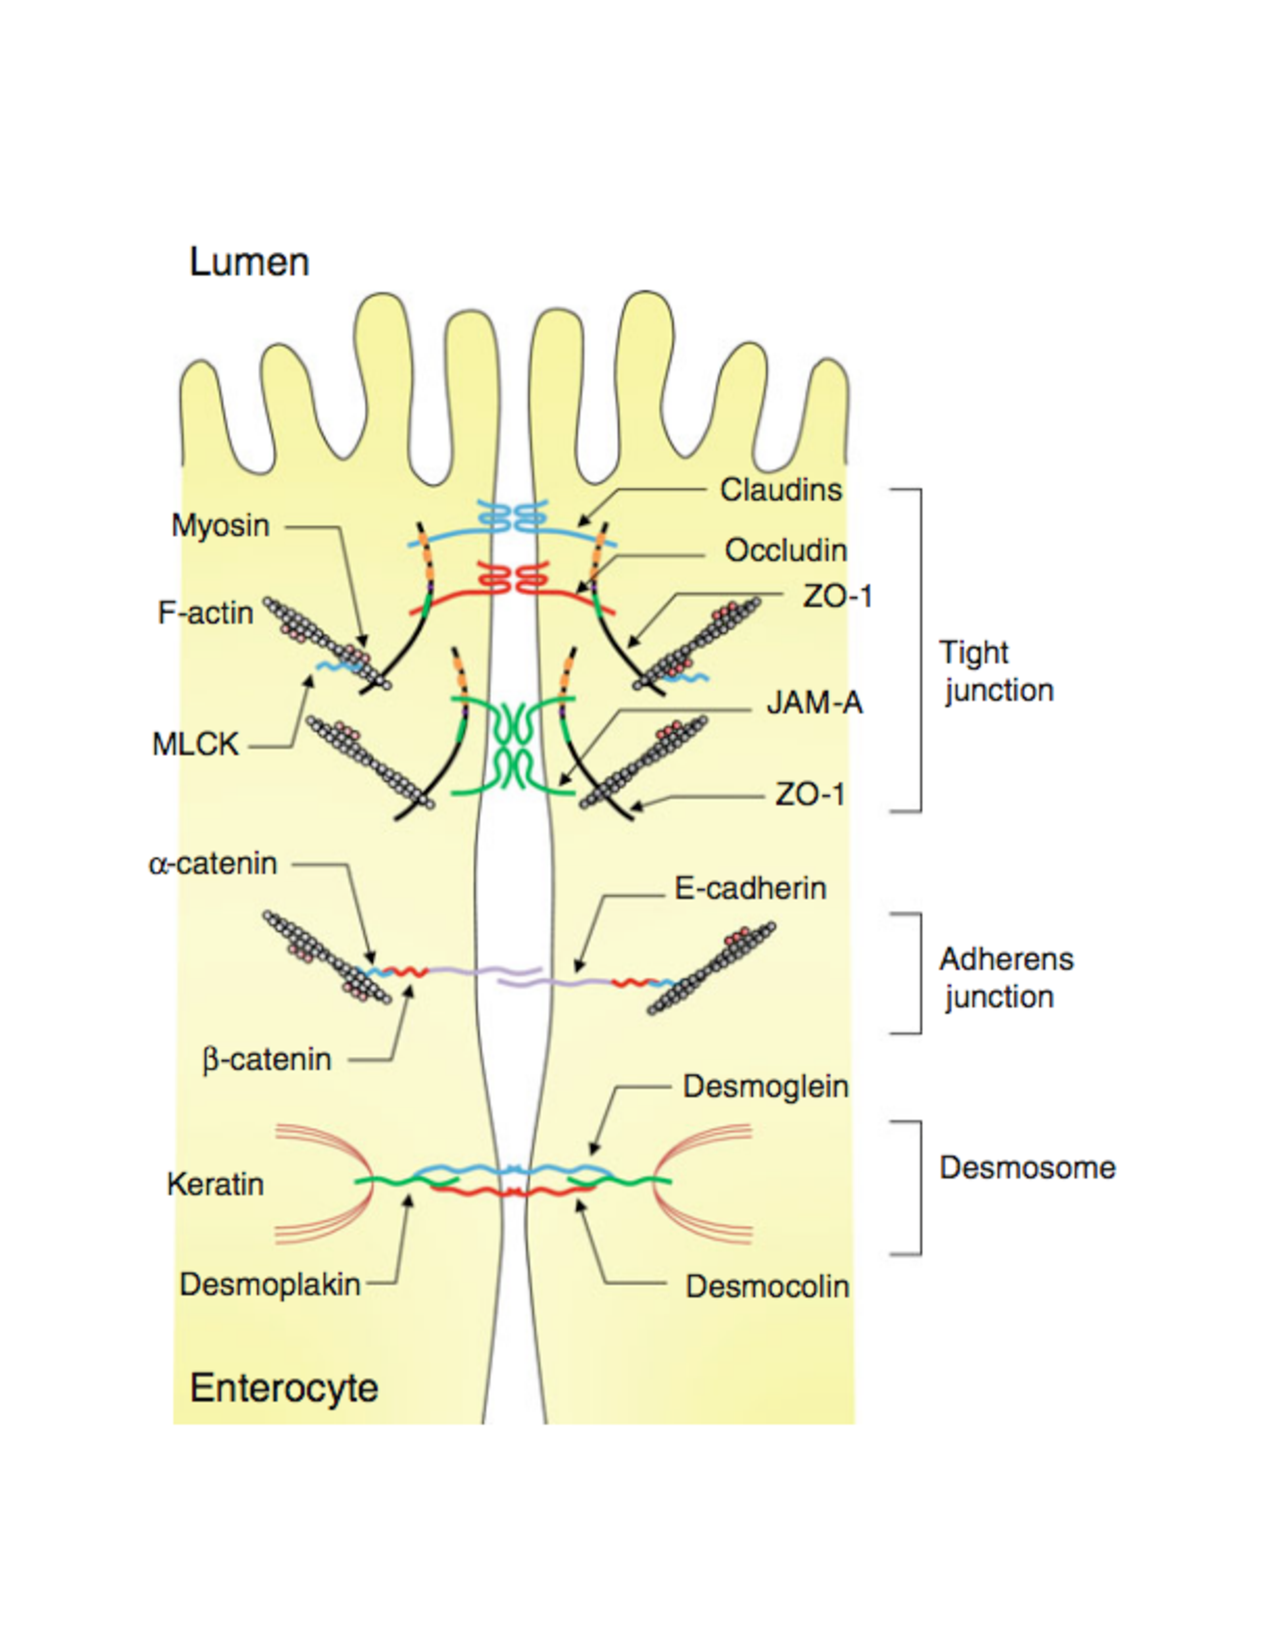
\includegraphics[height=3.5in]{tj}
	\caption{Schematic representation of the molecular structure of the intercellulat junction of intestinal epithelial cells. Taken from Suzuki (2013).}
	\label{fig:01}
	\end{figure}

Beyond this, various cells of the intestinal epithelium secrete a number of antimicrobial peptides that result in effective mucosal protection against pathogenic gut microbiota and prevent or greatly reduce the harmful translocation of these microbes across the gut barrier \cite{Ostaff:2013}.
	
\end{exercise}

\begin{exercise}[Exercise]{3} As we learned in the inflammation block and assigned reading, there is quite a bit of discussion in the field of cancer biology regarding the role of inflammation in tumorigenesis. On one side of the debate, it can be argued that inflammation drives tumorigenesis (causation). However, the opposing side would argue that inflammation is simply an enabling characteristic of cancer that occurs due to the loss of immune system homeostasis driven by the tumor (correlation). Design an experiment or series of studies to resolve this debate.\\

In colorectal cancer, it has been observed that mutant p53 (typically a tumor suppressor) promotes sustained NF-$\kappa$B activation, which in turn may promote pro-inflammatory cytokines such as IL-23 and IL-17 \cite{Dibra:2014}. A simple test of the role of inflammation in tumorigenesis here might involve the induction of a deliberate p53R172H mutation along with the administration of a $\beta$-Trcp antagonist. Such would result in normal NF-$\kappa$B activation (any upregulation by p53 would be counteracted by the $\beta$-Trcp antagonist, resulting in no net change to NF-$\kappa$B activation) and thereby no abnormal upregulation of pro-inflammatory pathways. If inflammation is necessary for tumorigenesis, there should be no observed tumor formation despite the presence of the p53 oncogene. Likewise, in an IL-17, IL-23 KO or knockdown mouse, there should be no tumor formation despite elevated NF-$\kappa$B activation. This would additionally evidence that tumorigenesis is specifically dependent on a pro-inflammatory cytokine milieu rather than simply increased NF-$\kappa$B activation.

In either case, tumorigenesis should occur immediately following the restoration of pro-inflammatory signaling. If, alternately, inflammation is only an enabling but not necessary characteristic for tumorigenesis, even upon removal of the pro-inflammatory response, tumor growth should be observed, although perhaps to a lesser extent than in inflamed conditions.

\end{exercise}

\begin{exercise}[Exercise]{4} Using murine models, design an \textit{in vivo} experiment to find out the pathogenic roles of B cells in SLE.  Describe the rationale of your study, a hypothesis, research strategies, anticipated results, potential pitfalls and solutions.\\

Systemic lupus erythematosus (SLE) is an autoimmune disorder in which autoantibody production results in chronic inflammatory damage to multiple host organ systems \cite{Dong:2011}. Emerging evidence suggests that populations of T\sub{H} cells produce IgG class-switched autoantibodies that contribute to the pathogenesis of lupus \cite{Datta:2005}. In such a model, stylized in Figure \ref{fig:02}, we see inappropriate T\sub{H} cell activation following recognition by B cells (or other antigen presenting cells) of autoantigens and subsequent loading of those peptide epitopes onto MHCII molecules.

\begin{figure}[htp]
  \centering
    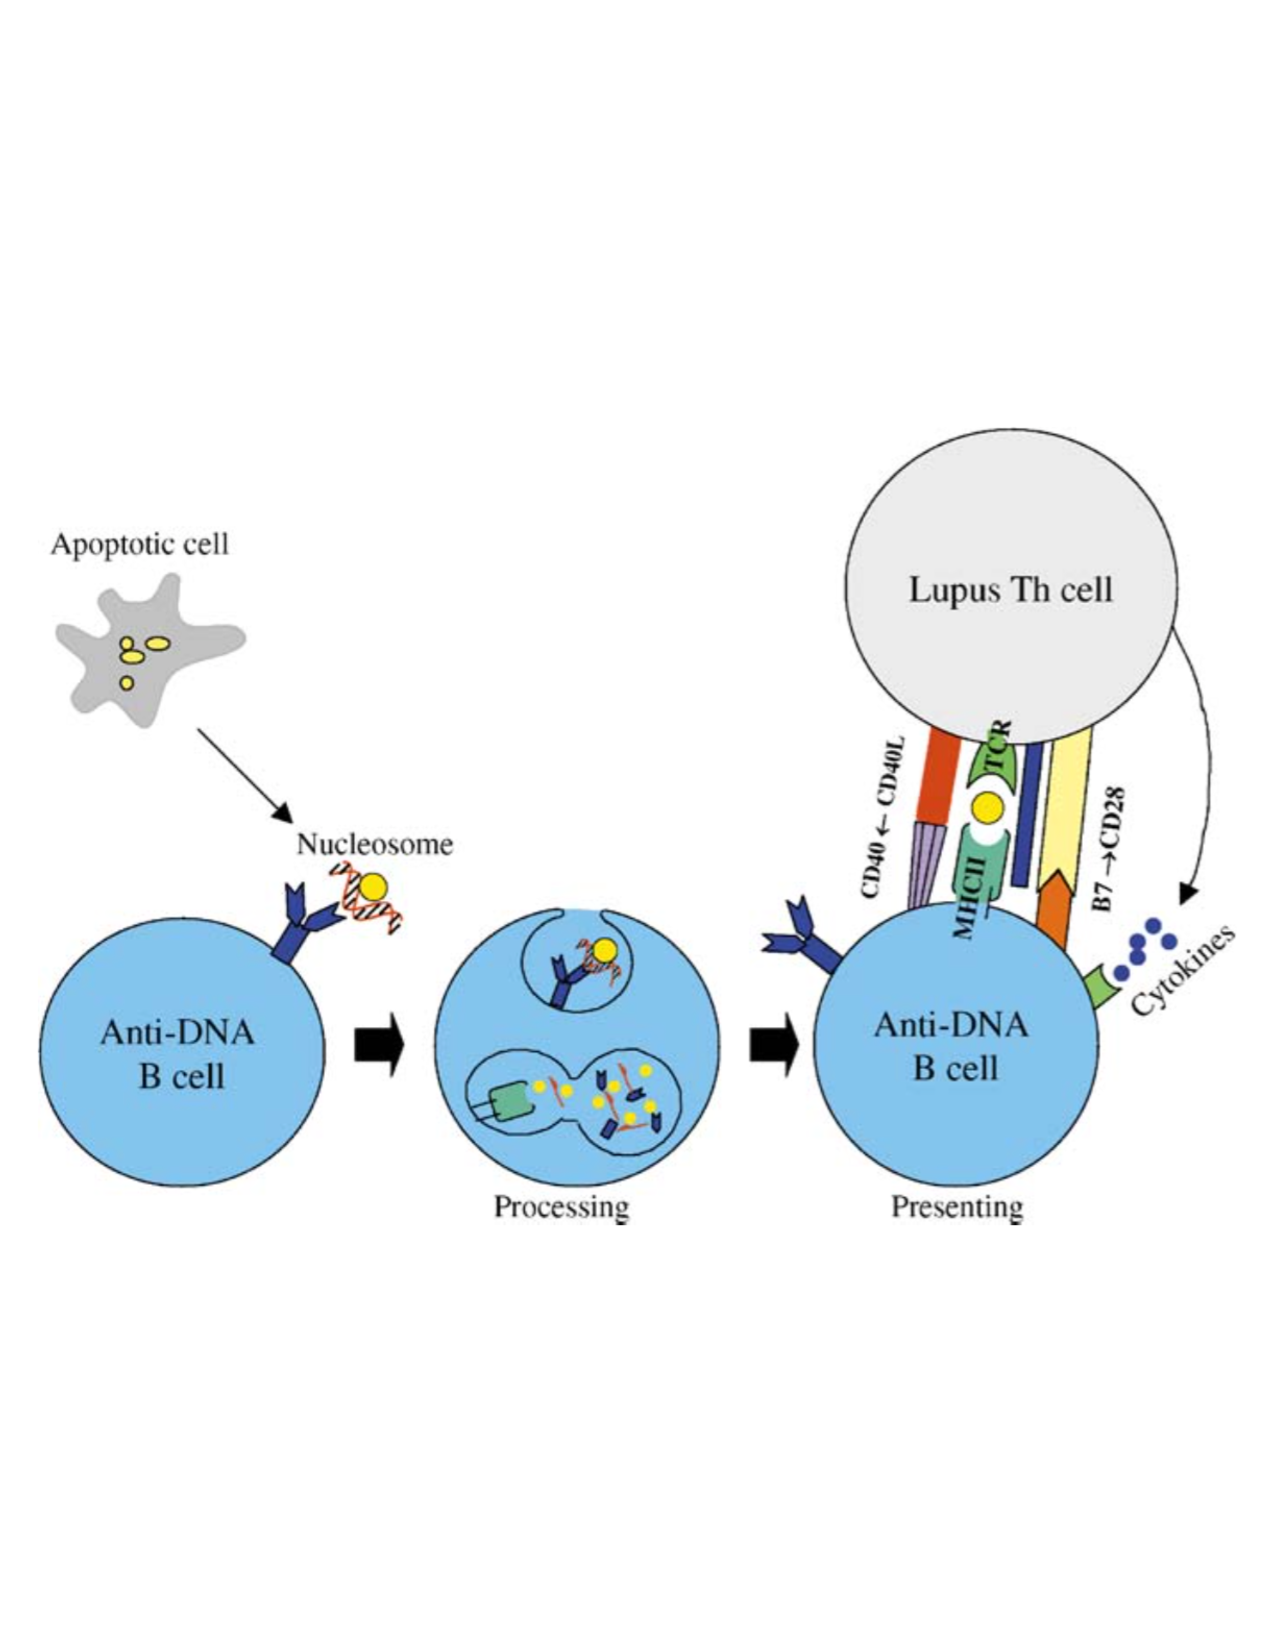
\includegraphics[width=0.65\textwidth]{sensitization}
	\caption{Stylized representation of inappropriate T\sub{H} cell activation following B cell sensitization to autoantigens. Taken from Datta, Zhang, and Xu (2005).}
	\label{fig:02}
\end{figure}

Further, it has been hypothesized that T\sub{FH} cell populations play a significant role in the loss of tolerance for self-reactive B cells at germinal centers: whereas self-reactive B cells would normally be excluded by germinal centers, the overabundance of T\sub{FH} cells may help to promote the survival of these B cell populations \cite{Dong:2011}.

Given the wide variety of immune interactions that have to date been shown to contribute to SLE pathogenesis, it seems unlikely that there can be a single experiment to adequately elucidate the roles of B cells in this process. However, we can ultimately reduce this to ``the proliferation of self-reactive B cells.''

On this understanding, should we want to simply evidence that B cell dysfunction is necessary (though likely not sufficient) for SLE pathogenesis, we might design an experiment in a murine model to address the role of tolerance checkpoints. Work by \citeauthor{Tiller:2007} has shown that IgG$^{+}$ memory B cells produce autoreactive antibodies, mostly derived \textit{de novo} during somatic hypermutation \citeyear{Tiller:2007}. This points to, and is further supported by work by \citeauthor{Cappione:2005}, errors in exclusion of autoreactive B cells from germinal centers contributing to SLE pathogenesis \citeyear{Cappione:2005}.

On this basis, we might hypothesize that by inhibiting or otherwise disrupting those checkpoints that would, in a healthy individual, exclude these autoreactive B cells, we would see the emergence of a lupus-like phenotype.

Experimentally, we might take a population of healthy mice and induce in one subpopulation a, for example, R620W polymorphism in PTPN22/Lyp which is known to decrease B cell receptor signaling at one such crucial tolerance checkpoint. Likewise,  IRAK4-, MYD88-, and UNC-93B-deficient mice could be generated and changes in phenotype observed \cite{Meffre:2011}. If indeed dysregulation of B cell tolerance checkpoints is necessary for SLE pathogenesis, we would expect these mice to begin to exhibit SLE-like symptoms. To confirm the role of B cells in this pathology, the affected mice could be then screened for elevated levels of autoreactive antibodies relative to the healthy baseline mouse.

\end{exercise}

\begin{exercise}[Exercise]{5} Please design an experiment to test, specifically, the contribution of T regulatory cells in the pathogenesis of sepsis in an animal model.\\

Regulatory T (Treg) cells are primarily responsible for shutting down the immune response following successful clearance of an invading pathogen \cite{Shevach:2000}. Further, it has been demonstrated that, although there does not appear to be an obvious role of Treg cells following the immediate onset of sepsis, the presence of competent Tregs is crucial for ultimate recovery from insult \cite{Kuhlhorn:2013}.

Given this understanding, to test the role of Tregs in sepsis, we might employ a DEREG (DEpletion of REGulatory T cells) murine model in which CD4$^{+}$Foxp3$^{+}$ Tregs can be rapidly and nearly completely ($\sim$95\% efficiency) depleted upon administration of diphtheria toxin. With such a model, we might deplete the animal's Treg cell population at various time points pre and post sepsis induction to first determine at what point Treg activation becomes crucial for sepsis response and resolution.

Following this, we might examine the role of, e.g., CD69 in T cell activation and proliferation \cite{Schmoeckel:2014}. In such an experiment, we might use an siRNA-mediated \textit{CD69}-knockdown to observe the downstream effects of incomplete Treg activation of the overall immune response to the septic insult. Likewise, a \textit{CD69}-knockin could be utilized to attempt to rescue the compromised immune response.

\end{exercise}

%%%%%%%%%%%%%%%%%%%%
%% REFERENCES
%%%%%%%%%%%%%%%%%%%%

\clearpage
\bibliographystyle{apacite}
\bibliography{references}

\end{document}